This work was presented at the IEEE International Symposium on Biomedical Imaging 2021 and published as part of its proceedings \citep{carse2021unsupervised}.



\section{Introduction}
\label{sec:unsupervised_intro}
\subsection{Unsupervised Representation Learning for Images}
\label{subsec:unsupervised_for_medical}
As previously discussed in Section \ref{subsec:active_for_medical_image_analysis}, the application of modern deep learning algorithms has demonstrated significant improvements in digital pathology tasks such as nuclei detection and disease classification~\citep{litjens2017survey}. The ability to jointly learn deep representations and discriminative classifiers or regressors through end-to-end training allows for feature representations that are specifically tailored to a given task. However, this approach necessitates a significant amount of annotated data for adequate generalization, which poses a major challenge for digital pathology~\citep{madabhushi2016image} and other medical image analysis domains. In an effort to address this challenge, we previously explored the use of active learning (Chapter \ref{ch:active_learning}), however, the limitations of this approach were highlighted in Section \ref{sec:active_conclusion} and subsequently led to a focus on unsupervised representation learning as a means to extract information from unannotated images. Unsupervised representation learning can be utilized to improve generalization, decrease data dimensionality, improve computational performance, and initialize deep supervised learning models when access to annotated data is limited~\citep{bengio2013representation}.

\begin{figure}
	\begin{minipage}[b]{.4\linewidth}
		\centering
		\centerline{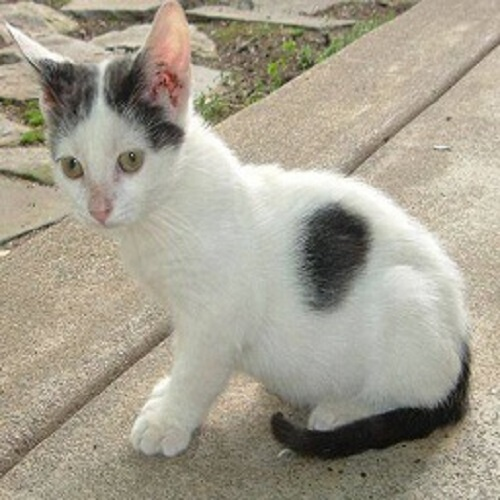
\includegraphics[width=\textwidth]{images/cat.jpg}}
		\centerline{(a)}\medskip
	\end{minipage}
	\hfill
	\begin{minipage}[b]{0.4\linewidth}
		\centering
		\centerline{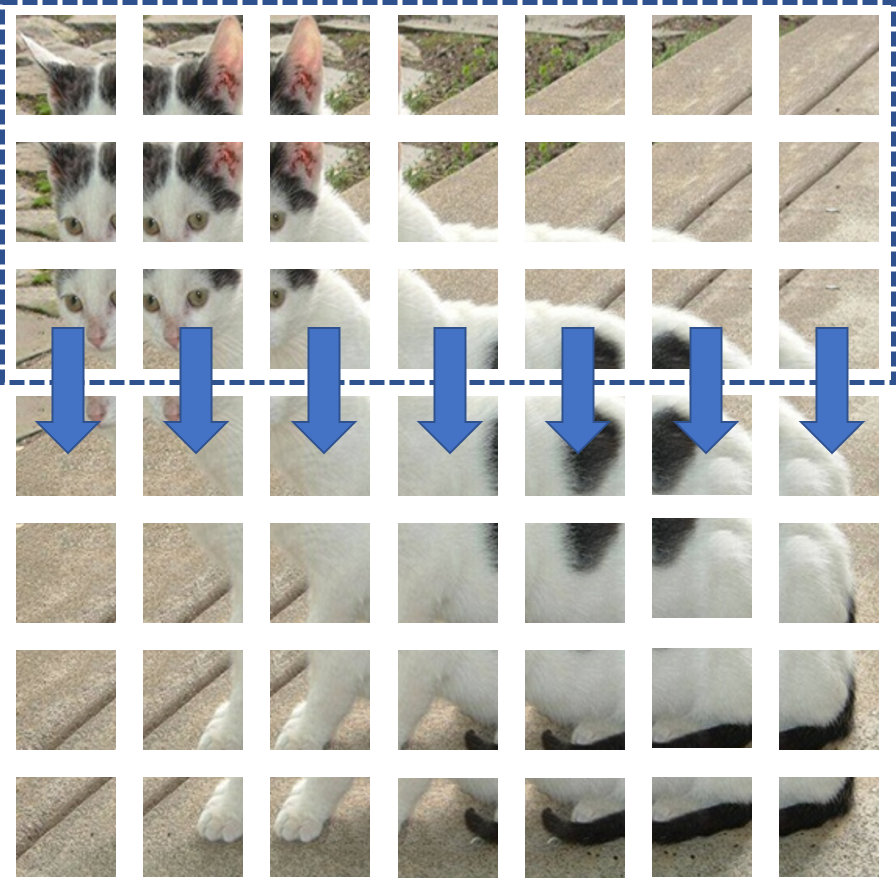
\includegraphics[width=\textwidth]{images/cat_grid_v2.png}}
		\centerline{(b)}\medskip
	\end{minipage}
	\\
	\begin{minipage}[b]{.4\linewidth}
		\centering
		\centerline{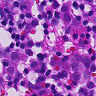
\includegraphics[width=\textwidth]{images/histo.png}}
		\centerline{(c)}\medskip
	\end{minipage}
	\hfill
	\begin{minipage}[b]{.4\linewidth}
		\centering
		\centerline{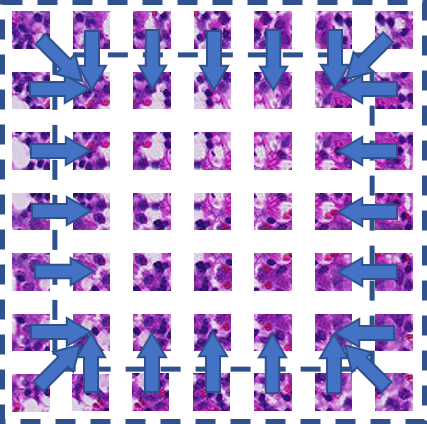
\includegraphics[width=\textwidth]{images/histo_grid.png}}
		\centerline{(d)}\medskip
	\end{minipage}
	\caption{(a) An example image from the ImageNet dataset~\citep{deng2009imagenet}. (b) Extracted overlapping patches with those used to produce context and autoregressor direction highlighted. (c) An example image from the Patch Camelyon dataset~\citep{veeling2018rotation}. (d) Extracted overlapping patches with those used to produce context and autoregressor direction highlighted.}
	\label{fig:example_cpc_patches}
\end{figure}

One approach to reducing the need for large, annotated datasets is through the use of transfer learning. This is accomplished by using the weights of a deep encoder, trained on a large pool of unannotated data, to initialize another model~\citep{weiss2016survey}. Contrastive predictive coding (CPC) is a state-of-the-art method for unsupervised representation learning~\citep{oord2018representation}. It involves training an autoregressive model to predict future data representations in a sequence, using a loss function composed of noise-contrastive estimation and importance sampling, to preserve the density ratio between each sample and their representation. Although originally developed for sequential data, CPC has been adapted for images by splitting each image into overlapping patches and using an encoder to produce a matrix of feature representations. A mask is then applied to the matrix so that an autoregressive model can only see a subset of the feature representations in order to predict the representations of the masked patches from the context available to it. This framework has been applied successfully to object detection and Imagenet classification tasks with modifications to model capacity, layer normalization, prediction directions, and patch-based augmentations~\citep{henaff2019data}. However, in previous implementations, the autoregressive model’s predictions were made in multiple directions individually, which can be inefficient when dealing with images, such as in digital pathology, where the orientation of the image is arbitrary and does not carry useful information. Figure~\ref{fig:example_cpc_patches}(b) illustrates an example of this framework applied to an image.

\subsection{Summary of Work}
\label{subsec:unsupervised_summary}
The current study builds upon the idea that unsupervised representation learning can be utilized to learn deep representations, which can then be used in conjunction with transfer learning to train a discriminative classifier with limited annotated data (as depicted in Figure~\ref{fig:active_unsupervised_learning_framework}). By implementing this approach, the need for complex deep learning-specific active learning query strategies is mitigated and instead allows for a focus on uncertainty-based querying. In order to realize this approach, a state-of-the-art unsupervised representation learning algorithm for digital pathology images was required. To this end, a multi-directional CPC extension was proposed, which includes an alternative mask for building latent context and a new extension to the autoregressive model PixelCNN~\citep{oord2016pixel} for multi-directional predictions (as depicted in Figure~\ref{fig:example_cpc_patches}(d)). The effectiveness of this modification was demonstrated using the PatchCamelyon dataset~\citep{veeling2018rotation}, derived from the Camelyon16 dataset~\citep{litjens20181399}, where it was shown that classification can be performed with less annotated data when utilizing representations learned in this way.

\begin{figure}
	\centering
	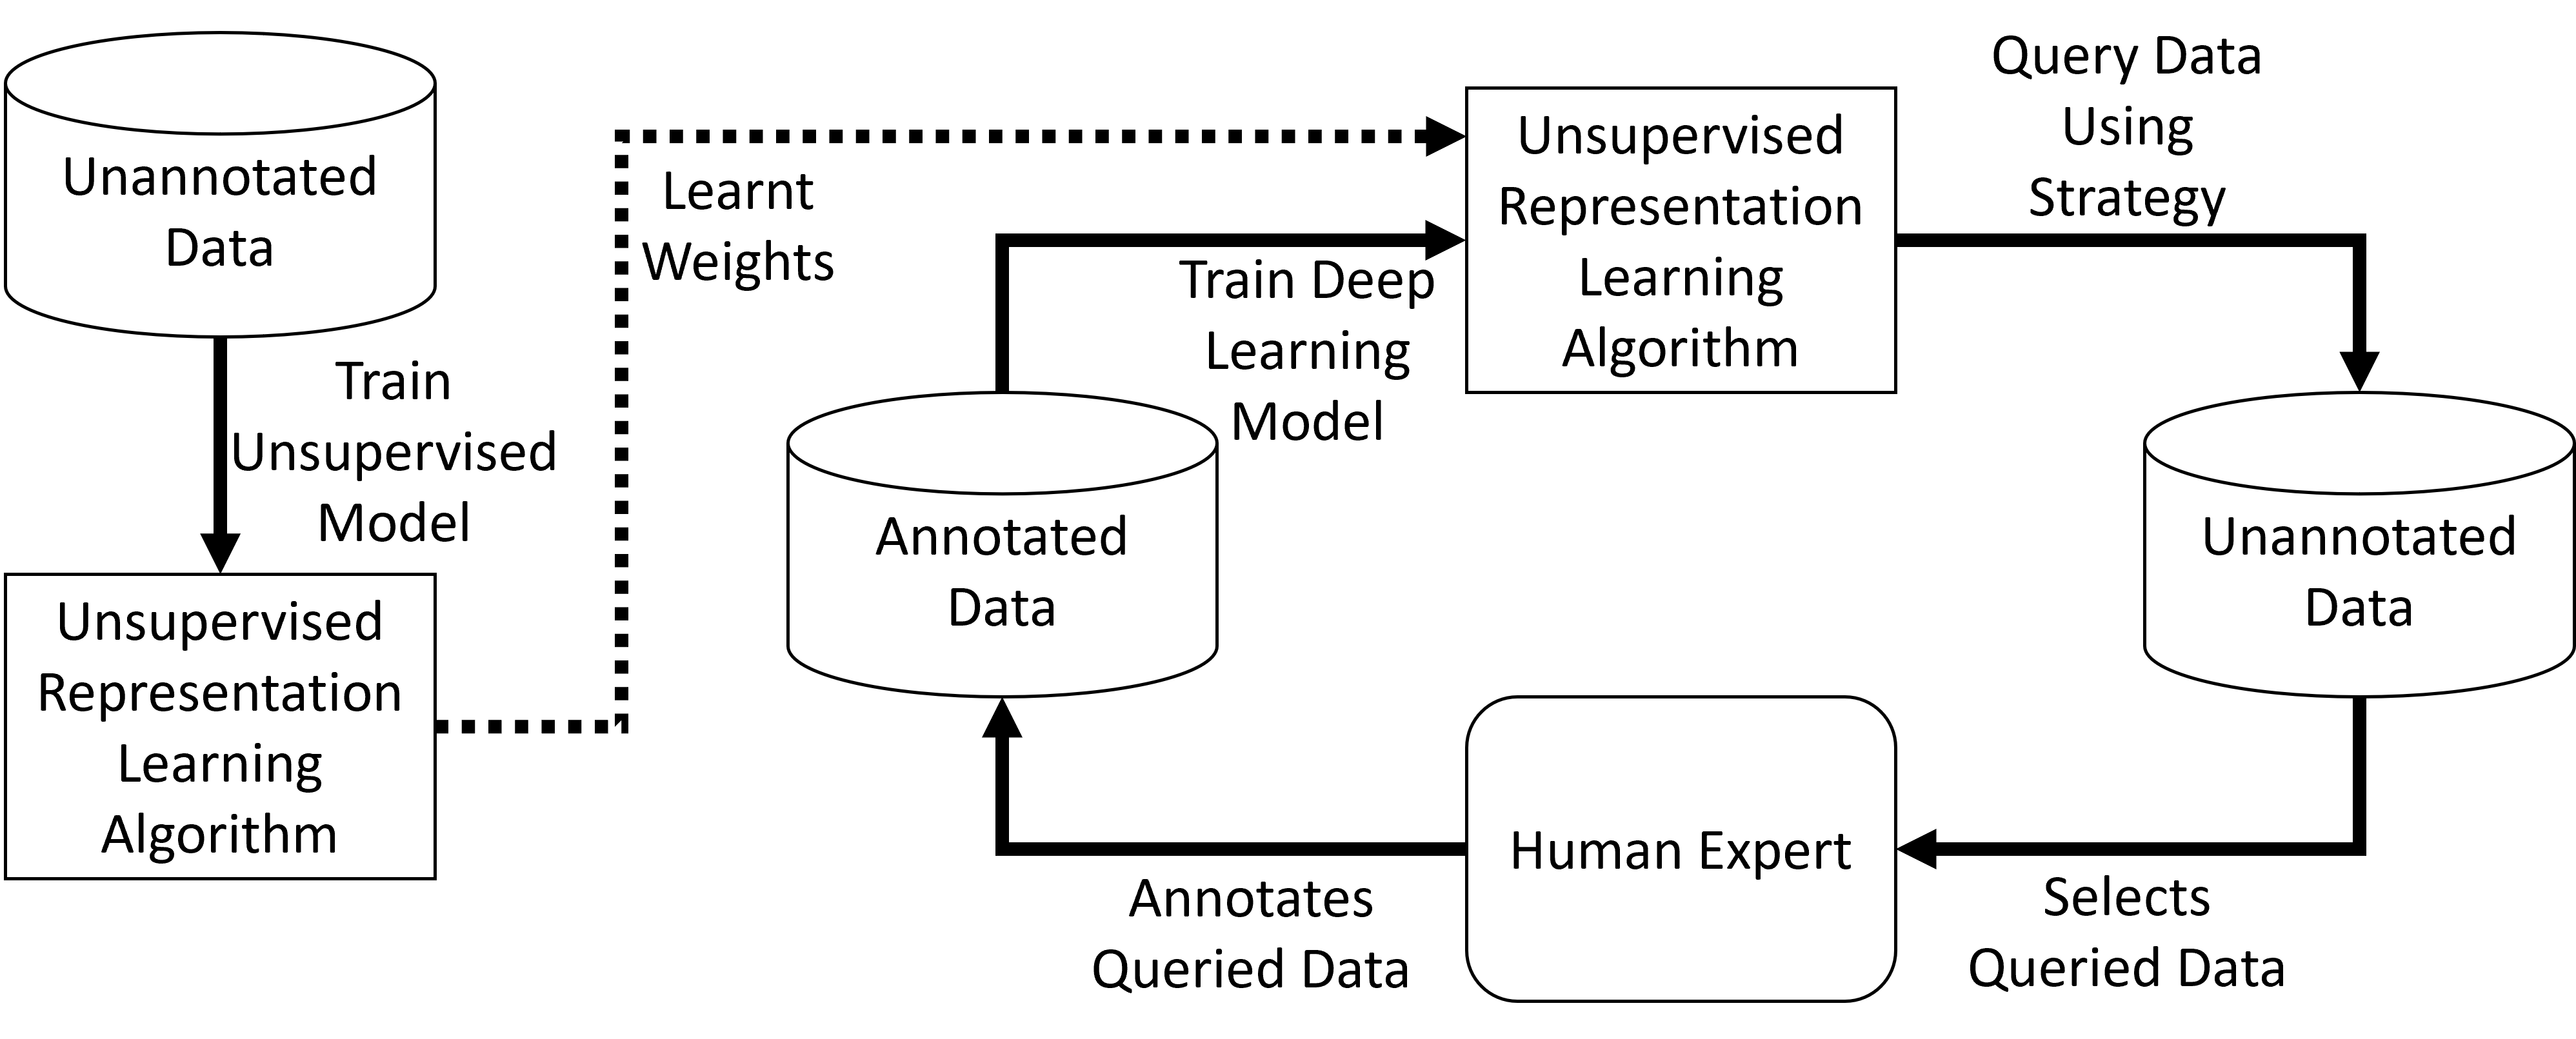
\includegraphics[width=\textwidth]{images/active_unsupervised_learning.png}
	\caption{Proposed active learning framework with learnt representations from unsupervised representation learning on unannotated data.}
	\label{fig:active_unsupervised_learning_framework}
\end{figure}



\section{Review of Deep Unsupervised Representation Learning}
\label{sec:unsupervised_review}
Review of Deep Unsupervised Representation Learning

\subsection{Unsupervised Representation Learning}
\label{subsec:unsupervised_representation}
Unsupervised Representation Learning

\subsection{Deep Unsupervised Representation Learning}
\label{subsec:unsupervised_deep_representation}
Deep Unsupervised Representation Learning

\subsection{Unsupervised Representation Learning for Medical Images}
\label{subsec:unsupervise_representation_for_medical}
Unsupervised Representation Learning for Medical Images



\section{Multi-Directional Contrastive Predictive Coding}
\label{sec:unsupervised_multi_directional_cpc}
Multi-Directional Contrastive Predictive Coding

\subsection{Contrastive Predictive Coding}
\label{subsec:unsupervised_cpc}
Contrastive Predictive Coding (CPC) is a method for learning feature representations in an unsupervised manner from sequential data. The CPC method is based on the idea of predicting future representations from past representations, thereby allowing the model to learn "slow" features that effectively represent the underlying input data distribution \citep{henaff2019data,oord2018representation}. A CPC model consists of two main components: an encoder $g_{en}$ that encodes each element $x_t$ of the input sequence $x$ into a latent representation $z_t = g_{en}(x_t)$, and an autoregressive model $g_{ar}$ that summarizes part of the latent representation sequence $z_{\le t}$ into a latent context representation $c_t = g_{ar}(z_{\le t})$. Instead of using the autoregressive model to predict future samples, a density ratio is modeled, which preserves the mutual information between $x_{t+k}$ and $c_t$ (as described in Equation\ref{eq:density_ratio}).

\begin{equation}
	f_k(x_{t+k}, c_t) \propto \frac{p(x_{t+k}|c_t)}{p(x_{t+k})}
	\label{eq:density_ratio}
\end{equation}

Direct evaluation of $p(x)$ or $p(x|c)$ is not possible, but since the distribution can be sampled, Noise-contrastive estimation \citep{gutmann2010noise} can be employed by comparing a target value to random negative samples. The loss function used to jointly optimize the encoder and autoregressive models is called InfoNCE (as described in Equation\ref{eq:InfoNCE}), it is based on Noise-contrastive estimation. The loss function uses a set $X={x_i,…,x_N}$ of $N$ random samples, containing one positive sample from $p(x_{t+k}|c_t)$ and $N-1$ negative samples from $p(x_{t+k})$. By optimizing this loss function, the result will be $f_k(x_{t+k}, c_t)$, which estimates the density ratio from Equation~\ref{eq:density_ratio}.

\begin{equation}
	L=-\underset{x}{\mathbb{E}}\left[\log\frac{f_k(x_{t+k},c_t)}{\sum_{x_j\in X}f_k(x_j,c_t))}\right]
	\label{eq:InfoNCE}
\end{equation} 

\subsection{Contrastive Predictive Coding for Computer Vision}
\label{subsec:unsupervised_cpc_for_vision}
Contrastive Predictive Coding (CPC) is a method originally proposed for sequential data, and its application to computer vision involves first dividing an input image into overlapping patches. Each patch is then encoded, and an autoregressive model is employed to generate a context vector from the patch representations at the top of the image (as depicted in Figure~\ref{fig:example_cpc_patches}(b), where the top 3 rows of patches were utilized~\citep{oord2018representation}). This approach treats each column of the image as a sequence, with the context vector from the top of the image used to model the density ratio with patch representations below. This technique has been demonstrated to achieve data-efficient results on high-level computer vision datasets, such as Imagenet, as shown in the study of~\cite{deng2009imagenet}.

\subsection{Multi-Directional Contrastive Predictive Coding}
\label{subsec:unsupervised_mdcpc}
The approach of treating columns of the representation matrix as individual sequences (as described in Section~\ref{subsec:unsupervised_cpc_for_vision}), can negatively impact performance when working with images where image orientation is irrelevant, such as histology patches or dermoscopic skin lesion images. While the orientation of certain histology whole slide images can be biologically meaningful, the orientation of image patches, such as those shown in Figure~\ref{fig:example_cpc_patches}(c) (sentinel lymph node) orientation, is not important. In such cases, the autoregressive model can struggle to predict patch representation from the provided context as the vertical image axis is arbitrary, unlike Imagenet where it correlates with the direction of gravity acting upon the image content.

\begin{figure}
	\centering
	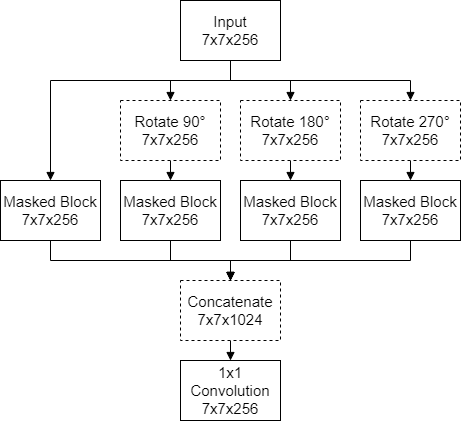
\includegraphics[width=0.9\textwidth]{mcb.png}
	\caption{Architecture of a Multi-Directional Masked Block}
	\label{fig:multi-directional_masked_block}
\end{figure}

To address this limitation, this work proposes two modifications inspired by image in-filling: an alternative latent mask for producing a context vector, and a modified PixelCNN~\citep{oord2016pixel} for multi-directional context building. The proposed multi-directional CPC utilizes these two modifications to more effectively learn representations from images where image rotation is uninformative.

The modified version of the PixelCNN is used as the autoregressive model in a multi-directional CPC model. This modification replaces each masked convolutional block of the PixelCNN architecture with a multi-directional masked block (Figure~\ref{fig:multi-directional_masked_block}). Each multi-directional masked block takes a single input image and by rotation 0, 90, 180 and 270 degrees, produces four versions of the original image. A masked block, as described in the paper from \cite{oord2016pixel}, is then applied to each of them. The four outputs from the masked blocks are then concatenated and put through a final 1x1 convolutional layer for dimensionality reduction.

This multi-directional autoregressive model is used to learn a latent context from multiple directions at the same time. To take advantage of this, an alternative latent mask inspired by in-filling is introduced. With this mask (illustrated in Figure~\ref{fig:example_cpc_patches}(d), the autoregressive model only has access to the patch representations around the perimeter of the patch representations. This means that images, where rotation is unimportant, can be better represented with features learned using a single directional CPC.



\section{Unsupervised Representation Learning Experiments}
\label{sec:unsupervised_experiments}
This section presents a comprehensive description of the datasets, training parameters, experimental setup, and results for the experimentation of the proposed multi-directional contrastive predictive coding approach on digital pathology whole slide patches. The methodology, experimental results and detailed information on the datasets used in this study are provided in a transparent and reproducible manner. The codes and full results used in this section can be accessed on the project's GitHub repository\footnote{GitHub Repository: \url{github.com/UoD-CVIP/Multi_Directional_CPC_Histology}} for further validation, replication and testing by the research community.

\subsection{Dataset}
\label{subsec:unsupervised_dataset}
In the experiments conducted, the publicly available dataset Patch Cameleyon~\citep{veeling2018rotation} was chosen for its suitability to evaluate the proposed method. This dataset was selected due to its larger number of non-overlapping whole slide image patches that possess no inherent directionality, making it a suitable benchmark for evaluating rotation-invariant representations, originally used to evaluate Rotation Equivariant CNNs~\citep{veeling2018rotation}. These patches were extracted from 400 whole slide image scans of sentinel lymph node sections from the Camelyon16 dataset~\citep{litjens20181399}. These whole slide images were collected from two different centres and digitized using an objective of 40x magnification, resulting in a pixel resolution of 0.243 microns. Each patch was annotated with a binary label indicating the presence or absence of metastatic tissue, by determining if the centre 32x32 pixels of the patch contains at least one pixel of tumour. The dataset contains a total of 327,680 patches which were split into training and testing sets, with a ratio of 90:10. To improve generalization, data augmentation was applied during training, by randomly rotating, flipping vertically and horizontally each patch during sampling.

\subsection{Experiment Setup}
\label{subsec:unsupervised_experiment}
In order to evaluate the proposed multi-directional contrastive predictive coding approach, an ablation study was conducted using different combinations of the single or multi-directional autoregressive models, and top-down or in-filling style latent masks. To evaluate the learned representations from the CPC models, the trained encoders were used to initialize the weights of 9 CNN classifiers. These CNN classifiers were then trained on a small, annotated subset of the training data, which was varied in size from 10 to 100,000 patches in logarithmic scale. The test set was held static across all experiments, and this was repeated 3 times, each time with a different subsample of the training data to validate the robustness of the results.

\subsection{Training Parameters}
\label{subsec:unsupervised_training}
In this study, the Contrastive Predictive Coding (CPC) models were trained using a method that involved splitting each input image into overlapping 24x24 patches that were overlapped by 12 pixels. A ResNeXt architecture~\citep{xie2017aggregated} with 101 layers was utilized as the encoder, followed by an additional convolutional layer to produce a 128-dimensional feature vector for each 24x24 patch in the image. The autoregressive model of the CPC was composed of 6 masked convolutional blocks to produce the context vector and predict the masked feature vectors. Additionally, 16 randomly selected images were used as negative samples for the CPC InfoNCE loss function.

The Adam optimization algorithm was utilized to train the CPC and CNN models, with an initial learning rate of 1e-4. The Adam optimizer~\citep{kingma2014adam} is based on adaptive estimation of first and second-order moments in the parameter gradients to adjust the learning rate during training. The CPC model was trained for 10 epochs with a batch size of 64 and the CNN models were trained over 50 epochs with a batch size of 258. 20\% of the available training data was used as the validation set to prevent overfitting, and early stopping was implemented by saving the model when the loss was lowest on the validation set.

The CPC models took an average of 33 hours to train using a single Nvidia GeForce RTX 2080 Ti~\footnote{NVIDIA GeForce RTX 2080 Ti: \url{www.nvidia.com/en-gb/geforce/20-series/}} using 16-bit precision. The training loss over the epochs (Figure~\ref{fig:cpc_training}) suggests that the use of a multi-directional autoregressive model was more efficient at reducing the InfoNCE loss than a single-directional top-down autoregressive model. The in-filling style latent mask in combination with the multi-directional autoregressive model stabilized the CPC training process.

\begin{figure}[h]
	\centering
	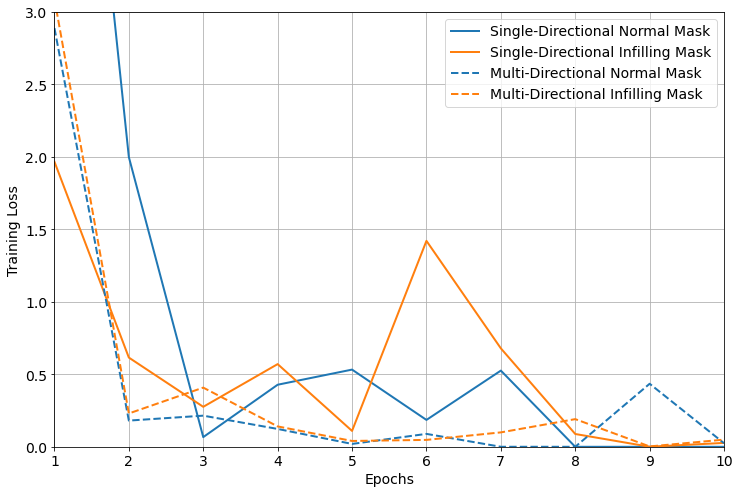
\includegraphics[width=\textwidth]{images/cpc_training.png}
	\caption{Training loss each epoch with the CPC Models.}
	\label{fig:cpc_training}
\end{figure}

\subsection{Results}
\label{subsec:unsupervised_results}
The results of the held-out testing set (32,768 images) for CNN classifiers trained using different CPC encoder's weights and biases for initialization are illustrated in Figure~\ref{fig:cpc_cnn_results} and Table~\ref{tab:cpc_cnn_results}. A baseline with CNN models that have had no pretraining was also included in the study. The findings indicate that the CNNs where small amounts of annotated data were used to train were able to achieve higher accuracies when a multi-directional autoregressive model is employed for initialization. In contrast, standard CPC struggled to learn a representation suitable for initializing a CNN classifier, sometimes resulting in lower accuracies compared to those initialized using random weights. The benefit of using the CPC pretraining decreases as the number of images increases, suggesting that this method of transfer learning is most effective when the number of annotated images is low.

\begin{figure}[h]
	\centering
	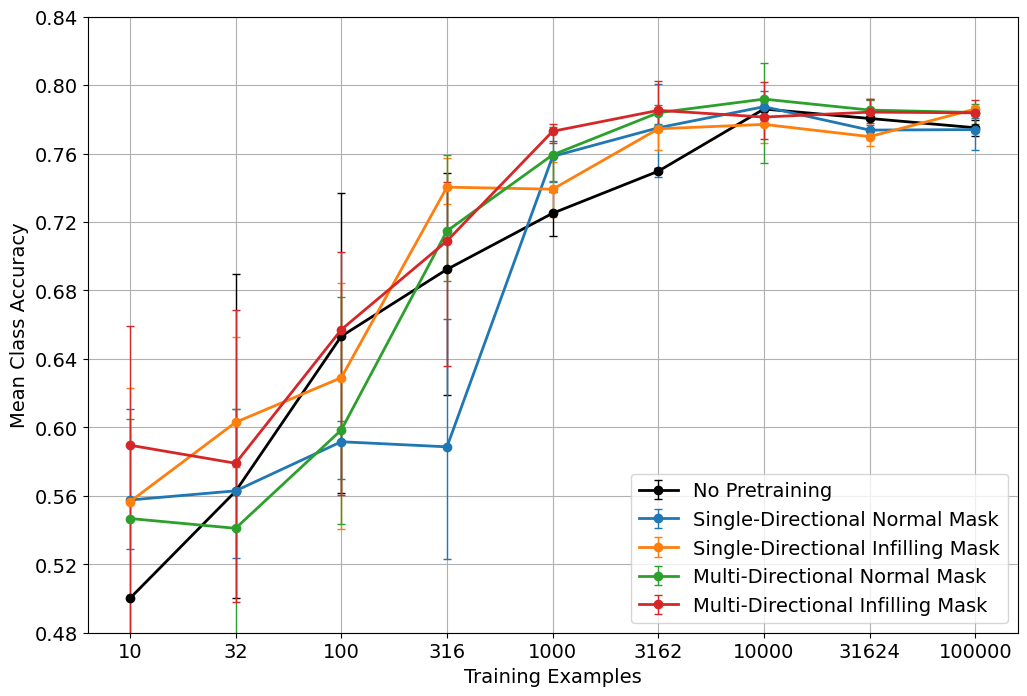
\includegraphics[width=\textwidth]{images/cpc_cnn_results.png}
	\caption{Mean class testing accuracies of the CNN classifiers trained using varying amounts of training examples, with standard errors.}
	\label{fig:cpc_cnn_results}
\end{figure}

\begin{table}[t]
	\centering
	\caption{Mean test accuracies of the CNN classifiers with different pre-training (standard deviation in parentheses).}
	\label{tab:cpc_cnn_results}
	\resizebox{\textwidth}{!}{%
		\begin{tabular}{r|rrrrr}
			\multicolumn{1}{c|}{\begin{tabular}[c]{@{}c@{}}Training\\ Examples\end{tabular}} &
			\multicolumn{1}{c}{\begin{tabular}[c]{@{}c@{}}No \\ Pretraining\end{tabular}} &
			\multicolumn{1}{c}{\begin{tabular}[c]{@{}c@{}}Single\\Directional\\Normal Mask\end{tabular}} &
			\multicolumn{1}{c}{\begin{tabular}[c]{@{}c@{}}Single\\Directional\\Infilling Mask\end{tabular}} &
			\multicolumn{1}{c}{\begin{tabular}[c]{@{}c@{}}Multi\\Directional\\Normal Mask\end{tabular}} &
			\multicolumn{1}{c}{\begin{tabular}[c]{@{}c@{}}Multi\\Directional\\Infilling Mask\end{tabular}} \\ \hline
			10     & 0.500 (0.000) & 0.561 (0.043)          & 0.561 (0.094)          & 0.546 (0.065)          & \textbf{0.582 (0.096)} \\
			32     & 0.563 (0.109) & 0.560 (0.045)          & \textbf{0.604 (0.043)} & 0.538 (0.082)          & 0.577 (0.086)          \\
			100    & 0.641 (0.125) & 0.590 (0.018)          & 0.636 (0.082)          & 0.595 (0.078)          & \textbf{0.655 (0.081)} \\
			316    & 0.694 (0.067) & 0.593 (0.109)          & \textbf{0.741 (0.014)} & 0.715 (0.039)          & 0.708 (0.062)          \\
			1000   & 0.727 (0.013) & 0.758 (0.014)          & 0.740 (0.016)          & 0.760 (0.016)          & \textbf{0.773 (0.006)} \\
			3162   & 0.750 (0.002) & 0.777 (0.028)          & 0.775 (0.012)          & 0.784 (0.006)          & \textbf{0.786 (0.014)} \\
			10000  & 0.786 (0.006) & 0.787 (0.008)          & 0.776 (0.012)          & \textbf{0.792 (0.033)} & 0.781 (0.019)          \\
			31624  & 0.779 (0.012) & 0.774 (0.004)          & 0.770 (0.009)          & \textbf{0.786 (0.005)} & 0.784 (0.009)          \\
			100000 & 0.775 (0.007) & 0.774 (0.011)          & \textbf{0.786 (0.003)} & 0.785 (0.006)          & 0.784 (0.010)
		\end{tabular}%
	}
\end{table}


\section{Conclusion}
\label{sec:conclusion}
The experimental results presented in Section~\ref{subsec:unsupervised_results} demonstrate that the original implementation of Contrastive Predictive Coding (CPC)~\citep{oord2018representation} does not perform well on patch-based digital pathology tasks. The proposed multi-directional modifications to the CPC, however, yielded better results and improved classification accuracies when annotated data were limited. These experiments illustrate that algorithms based on an assumption of image directionality, as is common in standard computer vision datasets such as CIFAR~\citep{krizhevsky2009learning} and ImageNet~\citep{deng2009imagenet}, may not perform well on images without such directionality. The results of this study suggest that the proposed multi-directional CPC method can be applied to other visual tasks where image orientation is unimportant, as is the case in multiple biomedical imaging settings.